% SOMAFOAM tutorial for new users: plasma fluid modelling basics and a first
% capacitively coupled plasma (CCP) run.
%   pdflatex somafoam_ccp_tutorial.tex   (twice, for the outline)
\documentclass[aspectratio=169,11pt]{beamer}
\usetheme{metropolis}
\usepackage{amsmath,amssymb}
\usepackage{booktabs}
\usepackage{tikz}
\usetikzlibrary{arrows.meta,positioning,decorations.pathreplacing}
\usepackage{listings}

\lstset{basicstyle=\ttfamily\scriptsize, columns=fullflexible, keepspaces=true,
        frame=single, rulecolor=\color{gray!60}, backgroundcolor=\color{gray!8},
        showstringspaces=false, breaklines=true}
\newcommand{\kw}[1]{\texttt{#1}}
\newcommand{\Te}{T_\mathrm{e}}
\newcommand{\nel}{n_\mathrm{e}}

\title{Getting started with SOMAFOAM}
\subtitle{Plasma fluid modelling basics and your first capacitively coupled plasma}
\author{SOMAFOAM tutorial}
\date{Version 2.0}

\begin{document}

\begin{frame}
  \titlepage
\end{frame}

\begin{frame}{What you will learn}
  \begin{itemize}
    \item What a low-temperature plasma and a capacitively coupled plasma (CCP) are
    \item The fluid equations that SOMAFOAM solves, and where their input data come from
    \item How a SOMAFOAM case is organised
    \item Step by step: run a 1D argon CCP at 1~Torr, look at the results
    \item How to change the pressure, the gap, the voltage, the frequency and the gas temperature
    \item The mistakes that new users make most often, and how to avoid them
  \end{itemize}
  \vfill
  \small Prerequisites: a Linux shell, a little Python, and access to a computer
  with SOMAFOAM built (the Pinnacles cluster in the examples).
\end{frame}

\begin{frame}{Outline}
  \tableofcontents
\end{frame}

% ===========================================================================
\section{Plasma basics}

\begin{frame}{Low-temperature plasmas}
  \begin{itemize}
    \item A partially ionised gas: electrons, positive (and negative) ions and a large
          background of neutral atoms or molecules
    \item Ionisation fraction typically $10^{-7}$ to $10^{-3}$ at 0.01--1000~Torr
    \item The electrons are hot ($\Te \approx 1$--10~eV, i.e.\ $10^4$--$10^5$~K) while ions
          and gas stay near room temperature
    \item The electrons gain energy from the electric field and lose it in collisions
          that excite, ionise and dissociate the gas
    \item Uses: etching and deposition in chip fabrication, surface treatment,
          lighting, plasma medicine, flow control
  \end{itemize}
  \vfill
  \small 1~eV corresponds to 11\,604~K; in SOMAFOAM temperatures are in kelvin.
\end{frame}

\begin{frame}{The capacitively coupled plasma}
  \begin{columns}
    \column{0.55\textwidth}
    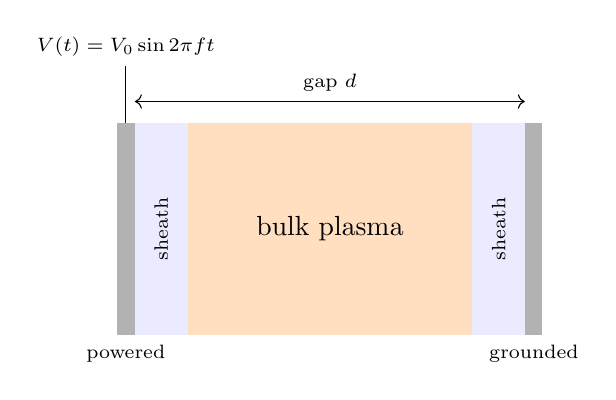
\begin{tikzpicture}[scale=0.9]
      \fill[gray!60] (0,0) rectangle (0.25,3);
      \fill[gray!60] (5.75,0) rectangle (6,3);
      \fill[blue!8] (0.25,0) rectangle (5.75,3);
      \fill[orange!25] (1.0,0) rectangle (5.0,3);
      \node at (3,1.5) {bulk plasma};
      \node[rotate=90] at (0.62,1.5) {\scriptsize sheath};
      \node[rotate=90] at (5.38,1.5) {\scriptsize sheath};
      \node[below] at (0.12,0) {\scriptsize powered};
      \node[below] at (5.88,0) {\scriptsize grounded};
      \draw[<->] (0.25,3.3) -- node[above] {\scriptsize gap $d$} (5.75,3.3);
      \draw (0.12,3) -- (0.12,3.8) node[above] {\scriptsize $V(t)=V_0\sin 2\pi f t$};
    \end{tikzpicture}
    \column{0.45\textwidth}
    \begin{itemize}\small
      \item Two parallel electrodes, one driven by an RF voltage (13.56--100~MHz)
      \item Quasi-neutral bulk: $\nel \approx n_\mathrm{i}$
      \item Sheaths: thin electron-depleted layers at the electrodes with strong
            fields that accelerate ions to the surfaces
      \item The sheaths expand and collapse every RF period, which heats the electrons
    \end{itemize}
  \end{columns}
\end{frame}

\begin{frame}{Scales you need to resolve}
  \begin{tabular}{lll}
    \toprule
    Quantity & Formula & Argon, $\nel=10^{16}$~m$^{-3}$, $\Te=2$~eV \\
    \midrule
    Debye length & $\lambda_\mathrm{D}=\sqrt{\varepsilon_0 k_\mathrm{B}\Te/(\nel e^2)}$ & $1.0\times10^{-4}$~m \\
    Electron plasma frequency & $\omega_\mathrm{pe}=\sqrt{\nel e^2/(\varepsilon_0 m_\mathrm{e})}$ & $5.6\times10^{9}$~rad/s \\
    Dielectric relaxation time & $\tau_\mathrm{d}=\varepsilon_0/(e\nel\mu_\mathrm{e})$ & $\sim10^{-12}$~s \\
    RF period at 40~MHz & $1/f$ & $2.5\times10^{-8}$~s \\
    \bottomrule
  \end{tabular}
  \vspace{1em}
  \begin{itemize}
    \item The cell size should be about $\lambda_\mathrm{D}$ or smaller, so that the
          sheaths are resolved by several cells
    \item The time step must resolve the RF period (hundreds of steps per period);
          SOMAFOAM's semi-implicit Poisson equation removes the dielectric-relaxation limit
    \item A discharge needs hundreds to thousands of periods to reach its periodic state
  \end{itemize}
\end{frame}

% ===========================================================================
\section{The fluid model}

\begin{frame}{Species continuity}
  For every transported species $k$ (electrons, ions, excited atoms):
  \begin{equation*}
    \frac{\partial n_k}{\partial t} + \nabla\cdot\boldsymbol{\Gamma}_k = S_k
  \end{equation*}
  \begin{itemize}
    \item $n_k$ number density [m$^{-3}$], $\boldsymbol{\Gamma}_k$ particle flux [m$^{-2}$s$^{-1}$]
    \item $S_k$ net production by the reactions [m$^{-3}$s$^{-1}$], for example for
          electrons from ionisation:
          \begin{equation*}
            S_\mathrm{e} = k_\mathrm{iz}(\Te)\,N\,\nel - \dots
          \end{equation*}
          with the gas density $N=p/k_\mathrm{B}T$ and a rate coefficient $k_\mathrm{iz}$ [m$^3$/s]
    \item Neutral species (metastables) only diffuse: $\boldsymbol{\Gamma}=-D\nabla n$
  \end{itemize}
\end{frame}

\begin{frame}{Drift--diffusion flux}
  \begin{equation*}
    \boldsymbol{\Gamma}_k = z_k\,\mu_k\,n_k\,\mathbf{E} - D_k\nabla n_k ,
    \qquad \mathbf{E}=-\nabla\Phi
  \end{equation*}
  \begin{itemize}
    \item $z_k$ charge number ($-1$ for electrons, $+1$ for Ar$^+$)
    \item Mobility $\mu_k$ [m$^2$V$^{-1}$s$^{-1}$] and diffusion coefficient $D_k$ [m$^2$/s]
    \item Both scale as $1/N$: tables give the products $\mu N$ and $DN$, so changing
          the pressure automatically rescales them
    \item Einstein relation, used for ions: $D_k=\mu_k k_\mathrm{B}T_k/e$
    \item Valid when collisions are frequent (pressures above about 50~mTorr); at lower
          pressure the momentum equation can be selected instead
  \end{itemize}
\end{frame}

\begin{frame}{Poisson's equation}
  \begin{equation*}
    \nabla\cdot(\varepsilon\nabla\Phi) = -e\sum_k z_k n_k
  \end{equation*}
  \begin{itemize}
    \item Couples the charged species through the electric field
    \item Boundary conditions: the applied voltage on the powered electrode,
          0 on the grounded one
    \item SOMAFOAM solves it semi-implicitly: the charge at the new time is predicted
          from the species fluxes, which allows time steps far above the
          dielectric relaxation time
    \item With dielectric layers (DBDs) the potential is solved in the dielectric regions
          as well and surface charge collects on their surfaces
  \end{itemize}
\end{frame}

\begin{frame}{Electron energy}
  \begin{align*}
    \frac{\partial}{\partial t}\Big(\tfrac32 k_\mathrm{B}\nel\Te\Big)
    + \nabla\cdot\Big(\tfrac52 k_\mathrm{B}\Te\boldsymbol{\Gamma}_\mathrm{e}
    - \kappa_\mathrm{e}\nabla\Te\Big)
    &= \underbrace{-e\,\boldsymbol{\Gamma}_\mathrm{e}\cdot\mathbf{E}}_{\text{Joule heating}}
    - \underbrace{\textstyle\sum_j \varepsilon_j k_j N\nel}_{\text{inelastic losses}} \\
    &\quad - \underbrace{3k_\mathrm{B}\tfrac{m_\mathrm{e}}{M}\nu_\mathrm{m}\nel(\Te-T)}_{\text{elastic losses}}
  \end{align*}
  \begin{itemize}
    \item Gives $\Te(x,t)$, and the rate coefficients and transport of the electrons
          are evaluated at the local $\Te$ (local mean energy approximation)
    \item $\varepsilon_j$ energy lost in reaction $j$ (15.76~eV for argon ionisation)
    \item Thermal conductivity $\kappa_\mathrm{e}=\tfrac52 k_\mathrm{B}\nel D_\mathrm{e}$
    \item Ions and gas: usually at the gas temperature (\kw{ion gasTemp}, \kw{gas none})
  \end{itemize}
\end{frame}

\begin{frame}{Reactions and rate coefficients}
  The argon set of the example (\kw{constant/reactions}):
  \begin{center}\small
  \begin{tabular}{lll}
    \toprule
    Process & Reaction & Rate \\
    \midrule
    elastic & e + Ar $\to$ e + Ar & table vs $\Te$ \\
    ionisation & e + Ar $\to$ 2e + Ar$^+$ & table, 15.76~eV \\
    excitation & e + Ar $\to$ e + Ar$^*$ & table, 11.56~eV \\
    stepwise ionisation & e + Ar$^*$ $\to$ 2e + Ar$^+$ & table, 4.43~eV \\
    quenching & e + Ar$^*$ $\to$ e + Ar & constant \\
    pooling & Ar$^*$ + Ar$^*$ $\to$ Ar$^+$ + Ar + e & constant \\
    two-body quenching & Ar$^*$ + Ar $\to$ 2Ar & constant \\
    \bottomrule
  \end{tabular}
  \end{center}
  \begin{itemize}\small
    \item Arrhenius form $k=AT^\beta e^{-T_a/T}$, or tables of $\ln k$ against $\Te$
    \item Units in the files: $k$ in m$^3$/(kmol\,s) and energies in J
  \end{itemize}
\end{frame}

\begin{frame}[fragile]{Where the electron data come from}
  \begin{itemize}
    \item The electron mobility, diffusion and rate coefficients depend on the electron
          energy distribution, which is not Maxwellian in general
    \item They are computed from cross sections (LXCat database, \url{www.lxcat.net}) by
          solving the Boltzmann equation of the electrons
    \item SOMAFOAM has its own solver, \kw{electronBoltzmann}, which writes the tables
          (\kw{mu\_electron}, \kw{D\_electron}, \kw{rate\_<n>}) in the format the solver reads
    \item Or use BOLSIG+ and convert its output
    \item Table format: two columns, $\Te$ [K] and $\mu N$ (or $\ln k$)
  \end{itemize}
  \begin{lstlisting}
(
529.008   0.1349E+27      // Te [K]   mu N [1/(V m s)]
568.362   0.1405E+27
...
  \end{lstlisting}
\end{frame}

\begin{frame}{Boundary conditions at the electrodes}
  \begin{itemize}
    \item Electrons (\kw{driftDiffusionElectronDensity}): thermal flux to the wall,
          $\Gamma_\mathrm{e}=\tfrac14\nel v_\mathrm{th}$, minus the secondary electrons
          emitted by ion impact, $\gamma\,\Gamma_\mathrm{i}$ (\kw{seec})
    \item Ions (\kw{driftDiffusionPositiveIonDensity}): drift into the wall when the field
          points into it
    \item Electron energy (\kw{electronTemperature}): energy carried by the wall flux and by the secondary electrons
    \item Metastables: quenched at the wall or zero gradient
    \item Potential: \kw{plasmaPotential} on the powered electrode (sinusoid, bias,
          waveforms), \kw{fixedValue 0} on the grounded one
  \end{itemize}
\end{frame}

\begin{frame}{Numerics in one slide}
  \begin{itemize}
    \item Finite volumes on a mesh of cells (1D, 2D, 3D, axisymmetric), built on foam-extend
    \item Implicit Euler in time with a fixed or adaptive step
    \item Drift--diffusion fluxes either with the standard schemes (\kw{Gauss limitedLinear})
          or with the Scharfetter--Gummel flux, which is exact for a constant field between
          two cell centres:
          \begin{equation*}
            \Gamma_f=\frac{D}{\Delta x}\big[B(-\mathrm{Pe})\,n_P-B(\mathrm{Pe})\,n_N\big],\quad
            \mathrm{Pe}=\frac{z\mu E\,\Delta x}{D},\quad B(x)=\frac{x}{e^x-1}
          \end{equation*}
    \item Each time step: Poisson $\rightarrow$ species $\rightarrow$ electron energy,
          optionally iterated to convergence with rejection of failed steps
    \item Verified against exact solutions: second order in space on uniform meshes,
          first order in time
  \end{itemize}
\end{frame}

% ===========================================================================
\section{SOMAFOAM cases}

\begin{frame}[fragile]{Building and the \kw{somafoam} command}
  On Pinnacles (once):
  \begin{lstlisting}
git clone https://github.com/vayyaswamy/SOMAFOAM.git
cd SOMAFOAM
scripts/somafoam submit build      # SLURM job, 1-2 h; log in logs/
scripts/somafoam env               # shows the paths that are used
  \end{lstlisting}
  Everyday commands:
  \begin{lstlisting}
scripts/somafoam list                      # all examples
scripts/somafoam run CASE --steps          # copy an example and run it
scripts/somafoam submit run CASE --steps   # the same as a SLURM job
scripts/somafoam test --short              # the test suite
  \end{lstlisting}
  \small \kw{--steps} runs the full example; without it an example that has an
  \kw{Allrun} (a test) runs only its short test. The run directory is
  \kw{/mnt/borgstore/\$USER/somafoam\_runs} on Pinnacles.
\end{frame}

\begin{frame}[fragile]{Anatomy of a case}
  \begin{columns}
    \column{0.5\textwidth}
    \begin{lstlisting}
case/
  0/                 initial and boundary
    Phi              conditions, one file
    electron         per field
    Arp1  Arm  Ar
    Te  T  Tion  p
  constant/          physics
    polyMesh/blockMeshDict   mesh
    plasmaProperties  species, models
    reactions         reaction list
    reaction_*        rate tables
    mu_electron  D_electron  mu_Arp1
    electroMagnetics  Poisson options
  system/            numerics, run control
    controlDict       times, output
    fvSchemes  fvSolution
    \end{lstlisting}
    \column{0.5\textwidth}
    \small
    \begin{itemize}
      \item \kw{0/}: one file per field with \kw{internalField} (initial value) and
            \kw{boundaryField} (one entry per boundary patch)
      \item \kw{constant/}: everything physical that does not change during the run
      \item \kw{system/}: time step, end time, output, discretisation schemes and
            linear solvers
      \item Results appear as new time directories, e.g.\ \kw{2.5e-07/}, holding
            the same fields
    \end{itemize}
  \end{columns}
\end{frame}

% ===========================================================================
\section{Your first CCP, step by step}

\begin{frame}{The example: 1~Torr argon CCP}
  \kw{examples/plasma/1TorrArgonPlasma/scharfetterGummel}
  \vspace{0.5em}
  \begin{center}
  \begin{tabular}{ll}
    \toprule
    Gas & argon, 1~Torr (133.3~Pa), 300~K \\
    Gap & 2~cm, 1D, 200 cells ($\Delta x=100~\mu$m) \\
    Drive & 100~V at 40~MHz on the electrode at $x=0$, ground at $x=2$~cm \\
    Species & e, Ar$^+$, Ar$^*$ (metastable), Ar background \\
    Time & step $10^{-10}$~s (250 per period), end $3~\mu$s (120 periods) \\
    Run time & about 20 minutes on one core \\
    \bottomrule
  \end{tabular}
  \end{center}
\end{frame}

\begin{frame}[fragile]{Step 1: run it}
  With the \kw{somafoam} command (it copies the case, makes the mesh and runs):
  \begin{lstlisting}
scripts/somafoam run plasma/1TorrArgonPlasma/scharfetterGummel --steps --tag first
  \end{lstlisting}
  or by hand in a copy of the case:
  \begin{lstlisting}
source etc/bashrc                      # SOMAFOAM environment
cp -r examples/plasma/1TorrArgonPlasma/scharfetterGummel ~/myCCP
cd ~/myCCP
blockMesh > log.blockMesh              # mesh from constant/polyMesh/blockMeshDict
somaFoam  > log.somaFoam 2>&1          # the solver; run from inside the case
  \end{lstlisting}
  \small Always start \kw{somaFoam} from inside the case directory: it reads the tables
  of \kw{constant/} by relative path.
\end{frame}

\begin{frame}[fragile]{Step 2: watch the run}
  \begin{lstlisting}
tail -f log.somaFoam
grep "Simulation Time" log.somaFoam | tail -1      # progress
  \end{lstlisting}
  \begin{itemize}
    \item Each step prints the solves of \kw{Phi}, the species and \kw{Te} with their residuals
    \item \kw{electrodes/0/electrode.dat}: voltage, conduction, displacement and total
          current of each electrode at every step
    \item Fields are written every \kw{writeInterval} (here $2.5\times10^{-7}$~s, 10 periods)
          into time directories
    \item \kw{...Mean} fields (\kw{N\_electronMean}, \kw{TeMean}) are averages over the
          interval since the previous write
  \end{itemize}
\end{frame}

\begin{frame}[fragile]{Step 3: look at the results}
  \begin{lstlisting}
# profiles at the last written time
postprocessing/plot_1d.py ~/myCCP --fields electron Arp1 Te Phi --times latest

# period-averaged profiles, metastables on a log axis
postprocessing/plot_1d.py ~/myCCP --fields N_electronMean TeMean Arm --log Arm

# how the discharge evolves (maximum, mean, mid-gap value per write)
postprocessing/plot_1d.py ~/myCCP --fields electron Arm Te --history --log Arm

# electrode voltage and current
postprocessing/plot_electrodes.py ~/myCCP --output current.png
  \end{lstlisting}
  \small \kw{--output file.png} saves the figure instead of showing it; \kw{--help} lists
  all options. ParaView also reads the case (\kw{touch case.foam}).
\end{frame}

\begin{frame}[fragile]{Step 4: is it converged?}
  \begin{itemize}
    \item An RF discharge starts from a guess and approaches a periodic state over
          hundreds to thousands of periods; metastables are the slowest
    \item Check the history plot: densities and $\Te$ should stop changing from one
          write to the next
    \item Continue a run: raise \kw{endTime} and set \kw{startFrom latestTime;}
    \item Stop automatically at the periodic state with \kw{convergenceStop} in
          \kw{system/controlDict}:
  \end{itemize}
  \small
\begin{verbatim}
convergenceStop
{
    fields      (N_electron N_Arm Te);
    window      1e-7;        // whole RF periods (4 at 40 MHz)
    tolerance   1e-4;        // relative change between windows
}
\end{verbatim}
\end{frame}

% ===========================================================================
\section{Changing the discharge}

\begin{frame}[fragile]{Changing the pressure}
  Example: 1~Torr $\rightarrow$ 0.5~Torr at 300~K, $N=p/k_\mathrm{B}T$:
  \begin{center}\small
  \begin{tabular}{lll}
    \toprule
    File & Entry & New value \\
    \midrule
    \kw{0/p} & \kw{internalField} & \kw{uniform 66.66;} [Pa] \\
    \kw{0/Ar} & \kw{internalField} & \kw{uniform 1.610E22;} [m$^{-3}$] \\
    \kw{constant/plasmaProperties} & \kw{Arm \{ D ... \}} & \kw{9.416e-3} (scales as $1/p$) \\
    \bottomrule
  \end{tabular}
  \end{center}
  \begin{itemize}\small
    \item \kw{0/p} and \kw{0/Ar} must agree: the chemistry takes the gas density from
          \kw{0/p}, so an inconsistent pair runs without error but gives wrong rates
    \item The electron and ion tables ($\mu N$, $DN$) rescale with $N$ by themselves
    \item A constant diffusion coefficient does not: scale it, or use
          \kw{diffusionModel pressureScaled; pD ...;} with $pD$ in Pa\,m$^2$/s
    \item Below about 0.1~Torr the sheaths widen and the drift--diffusion model becomes
          less accurate; check the cell size against the new Debye length
  \end{itemize}
\end{frame}

\begin{frame}[fragile]{Changing the gap}
  \kw{constant/polyMesh/blockMeshDict}: the vertices are multiplied by \kw{convertToMeters}
  \begin{lstlisting}
convertToMeters 2e-3;              // 10 units x 2 mm = 2 cm gap
vertices ( (0 0 0) (10 0 0) (10 1 0) (0 1 0)
           (0 0 1) (10 0 1) (10 1 1) (0 1 1) );
blocks ( hex (0 1 2 3 4 5 6 7) (200 1 1) simpleGrading (1 1 1) );
  \end{lstlisting}
  \begin{itemize}\small
    \item 3~cm gap: \kw{convertToMeters 3e-3;} and, to keep $\Delta x=100~\mu$m,
          \kw{(300 1 1)}
    \item Rerun \kw{blockMesh} after every change of the mesh
    \item The thickness in $y$ and $z$ (1 unit) does not matter in 1D (\kw{empty} patches),
          but the electrode currents in \kw{electrode.dat} are per this area
    \item \kw{simpleGrading (5 1 1)} grades the cells; for both sheaths use two blocks
          or the grading list of blockMesh
    \item Keep $\Delta x\lesssim\lambda_\mathrm{D}$ in the sheaths
  \end{itemize}
\end{frame}

\begin{frame}[fragile]{Changing the voltage and the frequency}
  \kw{0/Phi}, entry of the powered electrode:
  \begin{lstlisting}
electrode
{
    type            plasmaPotential;
    model           sinFrequencyModulated;   // V = amplitude sin(2 pi f t) + bias
    amplitude       uniform 100;             // [V]
    frequency       40E6;                    // [Hz]
    bias            0.0;                     // [V]
    value           uniform 0;
}
  \end{lstlisting}
  When the frequency changes, change \kw{system/controlDict} with it:
  \begin{itemize}\small
    \item \kw{deltaT}, \kw{deltaTMin}, \kw{deltaTMax}: keep 250 or more steps per period
          (13.56~MHz: $2.95\times10^{-10}$~s)
    \item \kw{writeInterval} and the averaging window: whole numbers of periods
    \item \kw{endTime}: lower frequencies need more time to reach the periodic state
  \end{itemize}
  \small Set power instead of voltage: boundary condition \kw{rfPowerElectrode} with a
  blocking capacitor (see the manual).
\end{frame}

\begin{frame}[fragile]{Other common changes}
  \begin{itemize}
    \item \textbf{Gas temperature}: \kw{0/T} and \kw{0/Tion}, then \kw{0/p} or \kw{0/Ar}
          so that $p=Nk_\mathrm{B}T$ still holds; the electron tables depend on $T$ only weakly
    \item \textbf{Secondary emission}: \kw{seec} in the electron and ion conditions of
          \kw{0/electron}, \kw{0/Arp1} and \kw{0/Te}
    \item \textbf{Initial plasma}: \kw{internalField} of \kw{0/electron} and \kw{0/Arp1}
          (equal, quasi-neutral), \kw{0/Te}; or profiles with \kw{setExpressionFields}
    \item \textbf{Flux scheme}: \kw{fluxScheme scharfetterGummel;} or \kw{fvSchemes} in
          \kw{constant/plasmaProperties}
    \item \textbf{Another gas}: new cross sections $\rightarrow$ \kw{electronBoltzmann}
          $\rightarrow$ new tables, a new \kw{constant/reactions}, ion mobility data
  \end{itemize}
  \begin{lstlisting}
// system/setExpressionFieldsDict: a cosine initial density
variables { L 0.02; profile "1e14 + 5e15*sin(3.14159265*x/L)"; }
fields    { electron "profile"; Arp1 "profile"; }
  \end{lstlisting}
\end{frame}

\begin{frame}[fragile]{Parameter studies}
  A script that makes one case per pressure from the example:
  \begin{lstlisting}
for mT in 250 500 1000; do
  dir=runs/p_$mT; cp -r examples/plasma/1TorrArgonPlasma/scharfetterGummel $dir
  p=$(python3 -c "print($mT*1e-3*133.3224)")
  N=$(python3 -c "print('%.4e' % ($mT*1e-3*133.3224/(1.380649e-23*300)))")
  sed -i "s/^internalField .*/internalField   uniform $p;/" $dir/0/p
  sed -i "s/^internalField .*/internalField   uniform $N;/" $dir/0/Ar
  # the metastable D of 4.7082e-3 m2/s is for 1 Torr
  D=$(python3 -c "print(4.7082e-3*1000/$mT)")
  sed -i "s/^\(\s*D\s*\)4.7082e-3;/\1$D;/" $dir/constant/plasmaProperties
  scripts/somafoam submit run $dir --steps --in-place
done
  \end{lstlisting}
  \small On a cluster, long runs are faster on the local disk of the node: the solver
  writes its log at every step (see the user guide).
\end{frame}

% ===========================================================================
\section{Pitfalls and next steps}

\begin{frame}{Common mistakes}
  \small
  \begin{tabular}{p{0.42\textwidth}p{0.52\textwidth}}
    \toprule
    Symptom & Cause and fix \\
    \midrule
    Rates far too fast or slow & \kw{0/p} and \kw{0/Ar} disagree; set both from $p=Nk_\mathrm{B}T$ \\
    \kw{cannot open constant/mu\_electron} & \kw{somaFoam} started outside the case; \kw{cd} into it \\
    The plasma dies out & time step too large for the start, initial density too low,
          or the voltage below the sustaining value \\
    $\Te$ grows without limit & an elastic reaction is listed but \kw{chemistry off}, so
          there is no elastic loss \\
    No output at the end time & \kw{writeInterval} longer than the run; write at \kw{endTime} \\
    Oscillating densities & cells larger than the Debye length; refine, or use
          Scharfetter--Gummel fluxes \\
    Results change with the step & not converged in time; halve \kw{deltaT} and compare \\
    \bottomrule
  \end{tabular}
\end{frame}

\begin{frame}{Exercises}
  \begin{enumerate}
    \item Run the 1~Torr example for 3~$\mu$s and plot $\nel$, $n_\mathrm{i}$ and $\Te$.
          Where are the sheaths, and how thick are they?
    \item Halve the pressure. How do the peak density and the sheath thickness change?
    \item Increase the gap to 3~cm with the same cell size. What happens to the peak density?
    \item Change the frequency to 13.56~MHz at the same voltage (adapt the time step!).
          Compare the electrode current amplitude.
    \item Run the \kw{defaultSchemes} variant and compare it with \kw{scharfetterGummel}.
    \item Extend a run with \kw{convergenceStop} until it is periodic. How many periods does
          the metastable density need?
  \end{enumerate}
\end{frame}

\begin{frame}{Where to go next}
  \begin{itemize}
    \item \kw{doc/USER\_GUIDE.md}: building, running, tests, SLURM, post-processing
    \item \kw{doc/manual/somafoam\_manual.pdf}: all equations, schemes, boundary conditions
    \item \kw{examples/README.md}: every example and what it shows
          \begin{itemize}\small
            \item \kw{plasma/100TorrArgonPlasma}: a higher-pressure discharge
            \item \kw{plasmaDielectric/ArgonDBD}: dielectric barrier discharge
            \item \kw{plasma/2DAdaptiveMeshArgon}: 2D with adaptive refinement
            \item \kw{zeroD/ArgonGlobal}: a global (0D) model, fast for chemistry studies
            \item \kw{plasma/HeliumIonDistribution}: ion energy distributions at the walls
            \item \kw{verification/}: cases with exact solutions, a good way to learn each model
          \end{itemize}
    \item Verma and Venkattraman, Comput.\ Phys.\ Commun.\ 263 (2021) 107855: the first SOMAFOAM paper
    \item Lieberman and Lichtenberg, \emph{Principles of Plasma Discharges and Materials Processing}
  \end{itemize}
\end{frame}

\end{document}
